\documentclass[]{article}
\usepackage{lmodern}
\usepackage{amssymb,amsmath}
\usepackage{ifxetex,ifluatex}
\usepackage{fixltx2e} % provides \textsubscript
\ifnum 0\ifxetex 1\fi\ifluatex 1\fi=0 % if pdftex
  \usepackage[T1]{fontenc}
  \usepackage[utf8]{inputenc}
\else % if luatex or xelatex
  \ifxetex
    \usepackage{mathspec}
  \else
    \usepackage{fontspec}
  \fi
  \defaultfontfeatures{Ligatures=TeX,Scale=MatchLowercase}
\fi
% use upquote if available, for straight quotes in verbatim environments
\IfFileExists{upquote.sty}{\usepackage{upquote}}{}
% use microtype if available
\IfFileExists{microtype.sty}{%
\usepackage{microtype}
\UseMicrotypeSet[protrusion]{basicmath} % disable protrusion for tt fonts
}{}
\usepackage[margin=1in]{geometry}
\usepackage{hyperref}
\hypersetup{unicode=true,
            pdftitle={Linea de tiempo},
            pdfauthor={Bernardo Ancidey},
            pdfborder={0 0 0},
            breaklinks=true}
\urlstyle{same}  % don't use monospace font for urls
\usepackage{color}
\usepackage{fancyvrb}
\newcommand{\VerbBar}{|}
\newcommand{\VERB}{\Verb[commandchars=\\\{\}]}
\DefineVerbatimEnvironment{Highlighting}{Verbatim}{commandchars=\\\{\}}
% Add ',fontsize=\small' for more characters per line
\usepackage{framed}
\definecolor{shadecolor}{RGB}{248,248,248}
\newenvironment{Shaded}{\begin{snugshade}}{\end{snugshade}}
\newcommand{\AlertTok}[1]{\textcolor[rgb]{0.94,0.16,0.16}{#1}}
\newcommand{\AnnotationTok}[1]{\textcolor[rgb]{0.56,0.35,0.01}{\textbf{\textit{#1}}}}
\newcommand{\AttributeTok}[1]{\textcolor[rgb]{0.77,0.63,0.00}{#1}}
\newcommand{\BaseNTok}[1]{\textcolor[rgb]{0.00,0.00,0.81}{#1}}
\newcommand{\BuiltInTok}[1]{#1}
\newcommand{\CharTok}[1]{\textcolor[rgb]{0.31,0.60,0.02}{#1}}
\newcommand{\CommentTok}[1]{\textcolor[rgb]{0.56,0.35,0.01}{\textit{#1}}}
\newcommand{\CommentVarTok}[1]{\textcolor[rgb]{0.56,0.35,0.01}{\textbf{\textit{#1}}}}
\newcommand{\ConstantTok}[1]{\textcolor[rgb]{0.00,0.00,0.00}{#1}}
\newcommand{\ControlFlowTok}[1]{\textcolor[rgb]{0.13,0.29,0.53}{\textbf{#1}}}
\newcommand{\DataTypeTok}[1]{\textcolor[rgb]{0.13,0.29,0.53}{#1}}
\newcommand{\DecValTok}[1]{\textcolor[rgb]{0.00,0.00,0.81}{#1}}
\newcommand{\DocumentationTok}[1]{\textcolor[rgb]{0.56,0.35,0.01}{\textbf{\textit{#1}}}}
\newcommand{\ErrorTok}[1]{\textcolor[rgb]{0.64,0.00,0.00}{\textbf{#1}}}
\newcommand{\ExtensionTok}[1]{#1}
\newcommand{\FloatTok}[1]{\textcolor[rgb]{0.00,0.00,0.81}{#1}}
\newcommand{\FunctionTok}[1]{\textcolor[rgb]{0.00,0.00,0.00}{#1}}
\newcommand{\ImportTok}[1]{#1}
\newcommand{\InformationTok}[1]{\textcolor[rgb]{0.56,0.35,0.01}{\textbf{\textit{#1}}}}
\newcommand{\KeywordTok}[1]{\textcolor[rgb]{0.13,0.29,0.53}{\textbf{#1}}}
\newcommand{\NormalTok}[1]{#1}
\newcommand{\OperatorTok}[1]{\textcolor[rgb]{0.81,0.36,0.00}{\textbf{#1}}}
\newcommand{\OtherTok}[1]{\textcolor[rgb]{0.56,0.35,0.01}{#1}}
\newcommand{\PreprocessorTok}[1]{\textcolor[rgb]{0.56,0.35,0.01}{\textit{#1}}}
\newcommand{\RegionMarkerTok}[1]{#1}
\newcommand{\SpecialCharTok}[1]{\textcolor[rgb]{0.00,0.00,0.00}{#1}}
\newcommand{\SpecialStringTok}[1]{\textcolor[rgb]{0.31,0.60,0.02}{#1}}
\newcommand{\StringTok}[1]{\textcolor[rgb]{0.31,0.60,0.02}{#1}}
\newcommand{\VariableTok}[1]{\textcolor[rgb]{0.00,0.00,0.00}{#1}}
\newcommand{\VerbatimStringTok}[1]{\textcolor[rgb]{0.31,0.60,0.02}{#1}}
\newcommand{\WarningTok}[1]{\textcolor[rgb]{0.56,0.35,0.01}{\textbf{\textit{#1}}}}
\usepackage{graphicx,grffile}
\makeatletter
\def\maxwidth{\ifdim\Gin@nat@width>\linewidth\linewidth\else\Gin@nat@width\fi}
\def\maxheight{\ifdim\Gin@nat@height>\textheight\textheight\else\Gin@nat@height\fi}
\makeatother
% Scale images if necessary, so that they will not overflow the page
% margins by default, and it is still possible to overwrite the defaults
% using explicit options in \includegraphics[width, height, ...]{}
\setkeys{Gin}{width=\maxwidth,height=\maxheight,keepaspectratio}
\IfFileExists{parskip.sty}{%
\usepackage{parskip}
}{% else
\setlength{\parindent}{0pt}
\setlength{\parskip}{6pt plus 2pt minus 1pt}
}
\setlength{\emergencystretch}{3em}  % prevent overfull lines
\providecommand{\tightlist}{%
  \setlength{\itemsep}{0pt}\setlength{\parskip}{0pt}}
\setcounter{secnumdepth}{0}
% Redefines (sub)paragraphs to behave more like sections
\ifx\paragraph\undefined\else
\let\oldparagraph\paragraph
\renewcommand{\paragraph}[1]{\oldparagraph{#1}\mbox{}}
\fi
\ifx\subparagraph\undefined\else
\let\oldsubparagraph\subparagraph
\renewcommand{\subparagraph}[1]{\oldsubparagraph{#1}\mbox{}}
\fi

%%% Use protect on footnotes to avoid problems with footnotes in titles
\let\rmarkdownfootnote\footnote%
\def\footnote{\protect\rmarkdownfootnote}

%%% Change title format to be more compact
\usepackage{titling}

% Create subtitle command for use in maketitle
\providecommand{\subtitle}[1]{
  \posttitle{
    \begin{center}\large#1\end{center}
    }
}

\setlength{\droptitle}{-2em}

  \title{Linea de tiempo}
    \pretitle{\vspace{\droptitle}\centering\huge}
  \posttitle{\par}
    \author{Bernardo Ancidey}
    \preauthor{\centering\large\emph}
  \postauthor{\par}
      \predate{\centering\large\emph}
  \postdate{\par}
    \date{23 de enero de 2020}


\begin{document}
\maketitle

\hypertarget{liberias}{%
\subsection{Liberías}\label{liberias}}

Se suben las librerías

\begin{Shaded}
\begin{Highlighting}[]
\KeywordTok{library}\NormalTok{(ggplot2)}
\KeywordTok{library}\NormalTok{(scales)}
\KeywordTok{library}\NormalTok{(lubridate)}
\end{Highlighting}
\end{Shaded}

\begin{verbatim}
## 
## Attaching package: 'lubridate'
\end{verbatim}

\begin{verbatim}
## The following object is masked from 'package:base':
## 
##     date
\end{verbatim}

\hypertarget{datos}{%
\subsection{Datos}\label{datos}}

Se cargan los datos:

\begin{verbatim}
##    month year                                   milestone      status
## 1      6 1818                          Correo del Orinoco     Cerrada
## 2      6 1827                                         UCV   Existente
## 3      1 1832                                         ULA   Existente
## 4      7 1833                         Biblioteca Nacional   Existente
## 5      1 1836               Archivo General de la Nación    Existente
## 6     10 1872                              Gaceta Oficial   Existente
## 7      2 1875 Museos de Bellas Artes y Ciencias Naturales   Existente
## 8      4 1881                 Teatro Municipal de Caracas   Existente
## 9      7 1883                  Teatro Baralt en Maracaibo   Existente
## 10     1 1886                       Teatro Puerto Cabello   Existente
## 11    10 1887           Academia Nacional de Bellas Artes   Existente
## 12    10 1894                             Teatro Valencia   Existente
## 13     6 1905                             Teatro Nacional   Existente
## 14     4 1917                 Protección patrimonial M.I.     Cerrada
## 15     6 1930             Orquesta Sinfónica de Venezuela   Existente
## 16     7 1936                 Radio Nacional de Venezuela   Existente
## 17     6 1936          Dir.de Cultura y Bellas Artes M.E.     Cerrada
## 18     6 1940        Dir. Cultura y Bienestar Social M.T.     Cerrada
## 19     6 1948                  Escuela Nacional de Ballet     Cerrada
## 20    11 1952                         Televisora Nacional   Existente
## 21     4 1960                                      INCIBA     Cerrada
## 22     5 1966            Cinemateca Nacional de Venezuela    Renovada
## 23     4 1968                        Monte Ávila Editores   Existente
## 24     7 1971           Conservatorio  Juan José Landaeta   Existente
## 25    11 1973                           Casa Andrés Bello   Existente
## 26    10 1974                                         GAN   Existente
## 27     9 1974                         Biblioteca Ayacucho   Existente
## 28     7 1974                                      CELARG   Existente
## 29     6 1975                 Conservatorio Simón Bolívar   Existente
## 30     8 1975                                       CONAC   Existente
## 31     4 1976                    Venezolana de Televisión   Existente
## 32     2 1976                       Teatro Teresa Carreño   Existente
## 33     2 1978             Fundación Musical Simón Bolívar   Existente
## 34    12 1982                           Librerías del Sur   Existente
## 35     5 1984                 Compañía Nacional de Teatro   Existente
## 36     3 1987                            Casa del Artista   Existente
## 37     5 1987                 Compañía Nacional de Música   Existente
## 38     9 1990           Centro de la Diversidad Cultural    Existente
## 39     9 1993            Instituto de Patrimonio Cultural   Existente
## 40     9 1993                                       CENAC   Existente
## 41    12 1996            Centro Nacional de la Fotografía   Existente
## 42     4 1997                                       CENAL   Existente
## 43     4 2005                           Museos Nacionales   Existente
## 44     5 2005                                 Red de Arte   Existente
## 45     7 2005                                      IARTES   Existente
## 46     7 2005                                        IAEM   Existente
## 47     2 2005                                        MPPC   Existente
## 48     3 2006                              Misión Cultura   Existente
## 49    12 2006                      Imprenta de la Cultura   Existente
## 50     6 2006                              Villa del Cine   Existente
## 51     2 2006      Distribuidora Venezolana de la Cultura   Existente
## 52    12 2006                                      CENDIS   Existente
## 53     2 2006                  Compañía Nacional de Danza   Existente
## 54     2 2006                              Amazonia Films   Existente
## 55     2 2006                Editorial El Perro y La Rana   Existente
## 56    10 2007                 Centro Nacional de Historia   Existente
## 57     5 2008                                     UNEARTE   Existente
## 58     1 2008                                 Alba Ciudad   Existente
## 59     8 2009                        Correo del Orinoco 2 Nueva Etapa
## 60     5 2013                   Editorial Alfredo Maneiro   Existente
## 61     9 2013                    Movimiento César Rengifo   Existente
## 62     8 2016                             Corazón Llanero   Existente
## 63     4 2017                              Corazón Urbano   Existente
## 64     2 2017                             Corazón Salsero   Existente
\end{verbatim}

Lo primero que haremos es definir una fecha para cada una de estas filas
como el día 1 del mes.

\begin{Shaded}
\begin{Highlighting}[]
\NormalTok{df}\OperatorTok{$}\NormalTok{date <-}\StringTok{ }\KeywordTok{with}\NormalTok{(df, }\KeywordTok{ymd}\NormalTok{(}\KeywordTok{sprintf}\NormalTok{(}\StringTok{'%04d%02d%02d'}\NormalTok{, year, month, }\DecValTok{1}\NormalTok{)))}
\NormalTok{df <-}\StringTok{ }\NormalTok{df[}\KeywordTok{with}\NormalTok{(df, }\KeywordTok{order}\NormalTok{(date)), ]}
\KeywordTok{head}\NormalTok{(df)}
\end{Highlighting}
\end{Shaded}

\begin{verbatim}
##   month year                     milestone    status       date
## 1     6 1818            Correo del Orinoco   Cerrada 1818-06-01
## 2     6 1827                           UCV Existente 1827-06-01
## 3     1 1832                           ULA Existente 1832-01-01
## 4     7 1833           Biblioteca Nacional Existente 1833-07-01
## 5     1 1836 Archivo General de la Nación  Existente 1836-01-01
## 6    10 1872                Gaceta Oficial Existente 1872-10-01
\end{verbatim}

A continuación se convierte el estado en una variable categórica
ordinal, en orden de criticidad que va de ``Existente a''Cerrada".
También definiremos algunos valores de color hexadecimales para
asociarlos a estos estados.

\begin{Shaded}
\begin{Highlighting}[]
\NormalTok{status_levels <-}\StringTok{ }\KeywordTok{c}\NormalTok{(}\StringTok{"Existente"}\NormalTok{, }\StringTok{"Renovada"}\NormalTok{, }\StringTok{"Nueva Etapa"}\NormalTok{, }\StringTok{"Cerrada"}\NormalTok{)}
\NormalTok{status_colors <-}\StringTok{ }\KeywordTok{c}\NormalTok{(}\StringTok{"#0070C0"}\NormalTok{, }\StringTok{"#00B050"}\NormalTok{, }\StringTok{"#FFC000"}\NormalTok{, }\StringTok{"#C00000"}\NormalTok{)}

\NormalTok{df}\OperatorTok{$}\NormalTok{status <-}\StringTok{ }\KeywordTok{factor}\NormalTok{(df}\OperatorTok{$}\NormalTok{status, }\DataTypeTok{levels=}\NormalTok{status_levels, }\DataTypeTok{ordered=}\OtherTok{TRUE}\NormalTok{)}
\end{Highlighting}
\end{Shaded}

En la línea de tiempo, se quiere variar la altura y la dirección de las
líneas, porque de lo contrario el texto de los hitos chocará. Se
necesita asignar las líneas y las alturas para que los hitos del mismo
mes sean los mismos, por lo que sólo se cambian los valores de altura y
posición.

A continuación, se ordena los datos por fecha y estado, de modo que el
estado ``cerrado''" se traza en último lugar y los colores que se
muestran son para el estado de los hitos cerrados.

\begin{Shaded}
\begin{Highlighting}[]
\NormalTok{positions <-}\StringTok{ }\KeywordTok{c}\NormalTok{(}\FloatTok{0.5}\NormalTok{, }\FloatTok{-0.5}\NormalTok{, }\FloatTok{1.0}\NormalTok{, }\FloatTok{-1.0}\NormalTok{, }\FloatTok{1.5}\NormalTok{, }\FloatTok{-1.5}\NormalTok{)}
\NormalTok{directions <-}\StringTok{ }\KeywordTok{c}\NormalTok{(}\DecValTok{1}\NormalTok{, }\DecValTok{-1}\NormalTok{)}

\NormalTok{line_pos <-}\StringTok{ }\KeywordTok{data.frame}\NormalTok{(}
    \StringTok{"date"}\NormalTok{=}\KeywordTok{unique}\NormalTok{(df}\OperatorTok{$}\NormalTok{date),}
    \StringTok{"position"}\NormalTok{=}\KeywordTok{rep}\NormalTok{(positions, }\DataTypeTok{length.out=}\KeywordTok{length}\NormalTok{(}\KeywordTok{unique}\NormalTok{(df}\OperatorTok{$}\NormalTok{date))),}
    \StringTok{"direction"}\NormalTok{=}\KeywordTok{rep}\NormalTok{(directions, }\DataTypeTok{length.out=}\KeywordTok{length}\NormalTok{(}\KeywordTok{unique}\NormalTok{(df}\OperatorTok{$}\NormalTok{date)))}
\NormalTok{)}

\NormalTok{df <-}\StringTok{ }\KeywordTok{merge}\NormalTok{(}\DataTypeTok{x=}\NormalTok{df, }\DataTypeTok{y=}\NormalTok{line_pos, }\DataTypeTok{by=}\StringTok{"date"}\NormalTok{, }\DataTypeTok{all =} \OtherTok{TRUE}\NormalTok{)}
\NormalTok{df <-}\StringTok{ }\NormalTok{df[}\KeywordTok{with}\NormalTok{(df, }\KeywordTok{order}\NormalTok{(date, status)), ]}

\KeywordTok{head}\NormalTok{(df)}
\end{Highlighting}
\end{Shaded}

\begin{verbatim}
##         date month year                     milestone    status position
## 1 1818-06-01     6 1818            Correo del Orinoco   Cerrada      0.5
## 2 1827-06-01     6 1827                           UCV Existente     -0.5
## 3 1832-01-01     1 1832                           ULA Existente      1.0
## 4 1833-07-01     7 1833           Biblioteca Nacional Existente     -1.0
## 5 1836-01-01     1 1836 Archivo General de la Nación  Existente      1.5
## 6 1872-10-01    10 1872                Gaceta Oficial Existente     -1.5
##   direction
## 1         1
## 2        -1
## 3         1
## 4        -1
## 5         1
## 6        -1
\end{verbatim}

Si hay múltiples hitos para un mes determinado, se necesita alterar
ligeramente sus posiciones (ligeramente más alto si está por encima de
la línea de tiempo y ligeramente más bajo si está por debajo).

Se puede hacer un recuento acumulativo de fechas individuales para
comprobar si se tienen múltiples hitos para un mes determinado.

\begin{Shaded}
\begin{Highlighting}[]
\NormalTok{text_offset <-}\StringTok{ }\FloatTok{0.05}

\NormalTok{df}\OperatorTok{$}\NormalTok{month_count <-}\StringTok{ }\KeywordTok{ave}\NormalTok{(df}\OperatorTok{$}\NormalTok{date}\OperatorTok{==}\NormalTok{df}\OperatorTok{$}\NormalTok{date, df}\OperatorTok{$}\NormalTok{date, }\DataTypeTok{FUN=}\NormalTok{cumsum)}
\NormalTok{df}\OperatorTok{$}\NormalTok{text_position <-}\StringTok{ }\NormalTok{(df}\OperatorTok{$}\NormalTok{month_count }\OperatorTok{*}\StringTok{ }\NormalTok{text_offset }\OperatorTok{*}\StringTok{ }\NormalTok{df}\OperatorTok{$}\NormalTok{direction) }\OperatorTok{+}\StringTok{ }\NormalTok{df}\OperatorTok{$}\NormalTok{position}
\KeywordTok{head}\NormalTok{(df)}
\end{Highlighting}
\end{Shaded}

\begin{verbatim}
##         date month year                     milestone    status position
## 1 1818-06-01     6 1818            Correo del Orinoco   Cerrada      0.5
## 2 1827-06-01     6 1827                           UCV Existente     -0.5
## 3 1832-01-01     1 1832                           ULA Existente      1.0
## 4 1833-07-01     7 1833           Biblioteca Nacional Existente     -1.0
## 5 1836-01-01     1 1836 Archivo General de la Nación  Existente      1.5
## 6 1872-10-01    10 1872                Gaceta Oficial Existente     -1.5
##   direction month_count text_position
## 1         1           1          0.55
## 2        -1           1         -0.55
## 3         1           1          1.05
## 4        -1           1         -1.05
## 5         1           1          1.55
## 6        -1           1         -1.55
\end{verbatim}

Como se quiere mostrar todos los meses en las líneas de tiempo, no sólo
los meses para los que hay eventos, se crear un dataframe que contenga
todos los meses.

Se empieza 2 meses antes del primer hito y se termina 2 meses después
del último hito para tener un poco de memoria intermedia.

\begin{Shaded}
\begin{Highlighting}[]
\NormalTok{month_buffer <-}\StringTok{ }\DecValTok{2}

\NormalTok{month_date_range <-}\StringTok{ }\KeywordTok{seq}\NormalTok{(}\KeywordTok{min}\NormalTok{(df}\OperatorTok{$}\NormalTok{date) }\OperatorTok{-}\StringTok{ }\KeywordTok{months}\NormalTok{(month_buffer), }\KeywordTok{max}\NormalTok{(df}\OperatorTok{$}\NormalTok{date) }\OperatorTok{+}\StringTok{ }\KeywordTok{months}\NormalTok{(month_buffer), }\DataTypeTok{by=}\StringTok{'month'}\NormalTok{)}
\NormalTok{month_format <-}\StringTok{ }\KeywordTok{format}\NormalTok{(month_date_range, }\StringTok{'%b'}\NormalTok{)}
\NormalTok{month_df <-}\StringTok{ }\KeywordTok{data.frame}\NormalTok{(month_date_range, month_format)}
\end{Highlighting}
\end{Shaded}

Se hace lo mismo para los años que también se quieren mostrar.

Sólo se mostrarán los años para los que hay un cruce de diciembre/enero,
esto es lo que está haciendo la línea de intersección (intersect).

\begin{Shaded}
\begin{Highlighting}[]
\NormalTok{year_date_range <-}\StringTok{ }\KeywordTok{seq}\NormalTok{(}\KeywordTok{min}\NormalTok{(df}\OperatorTok{$}\NormalTok{date) }\OperatorTok{-}\StringTok{ }\KeywordTok{months}\NormalTok{(month_buffer), }\KeywordTok{max}\NormalTok{(df}\OperatorTok{$}\NormalTok{date) }\OperatorTok{+}\StringTok{ }\KeywordTok{months}\NormalTok{(month_buffer), }\DataTypeTok{by=}\StringTok{'year'}\NormalTok{)}
\NormalTok{year_date_range <-}\StringTok{ }\KeywordTok{as.Date}\NormalTok{(}
    \KeywordTok{intersect}\NormalTok{(}
        \KeywordTok{ceiling_date}\NormalTok{(year_date_range, }\DataTypeTok{unit=}\StringTok{"year"}\NormalTok{),}
        \KeywordTok{floor_date}\NormalTok{(year_date_range, }\DataTypeTok{unit=}\StringTok{"year"}\NormalTok{)}
\NormalTok{    ),  }\DataTypeTok{origin =} \StringTok{"1970-01-01"}
\NormalTok{)}
\NormalTok{year_format <-}\StringTok{ }\KeywordTok{format}\NormalTok{(year_date_range, }\StringTok{'%Y'}\NormalTok{)}
\NormalTok{year_df <-}\StringTok{ }\KeywordTok{data.frame}\NormalTok{(year_date_range, year_format)}
\end{Highlighting}
\end{Shaded}

Ahora que se tienen los datos en un estado listo para ser trazados, se
puede armar el gráfico.

\begin{Shaded}
\begin{Highlighting}[]
\NormalTok{timeline_plot<-}\KeywordTok{ggplot}\NormalTok{(df,}\KeywordTok{aes}\NormalTok{(}\DataTypeTok{x=}\NormalTok{date,}\DataTypeTok{y=}\DecValTok{0}\NormalTok{, }\DataTypeTok{col=}\NormalTok{status, }\DataTypeTok{label=}\NormalTok{milestone))}
\NormalTok{timeline_plot<-timeline_plot}\OperatorTok{+}\KeywordTok{labs}\NormalTok{(}\DataTypeTok{col=}\StringTok{"Hitos"}\NormalTok{)}
\NormalTok{timeline_plot<-timeline_plot}\OperatorTok{+}\KeywordTok{scale_color_manual}\NormalTok{(}\DataTypeTok{values=}\NormalTok{status_colors, }\DataTypeTok{labels=}\NormalTok{status_levels, }\DataTypeTok{drop =} \OtherTok{FALSE}\NormalTok{)}
\NormalTok{timeline_plot<-timeline_plot}\OperatorTok{+}\KeywordTok{theme_classic}\NormalTok{()}

\CommentTok{# Trazar una línea negra horizontal para la línea de tiempo}
\NormalTok{timeline_plot<-timeline_plot}\OperatorTok{+}\KeywordTok{geom_hline}\NormalTok{(}\DataTypeTok{yintercept=}\DecValTok{0}\NormalTok{, }
                \DataTypeTok{color =} \StringTok{"black"}\NormalTok{, }\DataTypeTok{size=}\FloatTok{0.3}\NormalTok{)}

\CommentTok{# Trazar líneas de segmentos verticales para hitos}
\NormalTok{timeline_plot<-timeline_plot}\OperatorTok{+}\KeywordTok{geom_segment}\NormalTok{(}\DataTypeTok{data=}\NormalTok{df[df}\OperatorTok{$}\NormalTok{month_count }\OperatorTok{==}\StringTok{ }\DecValTok{1}\NormalTok{,], }\KeywordTok{aes}\NormalTok{(}\DataTypeTok{y=}\NormalTok{position,}\DataTypeTok{yend=}\DecValTok{0}\NormalTok{,}\DataTypeTok{xend=}\NormalTok{date), }\DataTypeTok{color=}\StringTok{'black'}\NormalTok{, }\DataTypeTok{size=}\FloatTok{0.2}\NormalTok{)}

\CommentTok{# Trazar los puntos de dispersión en cero y la fecha}
\NormalTok{timeline_plot<-timeline_plot}\OperatorTok{+}\KeywordTok{geom_point}\NormalTok{(}\KeywordTok{aes}\NormalTok{(}\DataTypeTok{y=}\DecValTok{0}\NormalTok{), }\DataTypeTok{size=}\DecValTok{3}\NormalTok{)}

\CommentTok{# No muestra los ejes, posiciona apropiadamente la leyenda}
\NormalTok{timeline_plot<-timeline_plot}\OperatorTok{+}\KeywordTok{theme}\NormalTok{(}\DataTypeTok{axis.line.y=}\KeywordTok{element_blank}\NormalTok{(),}
                 \DataTypeTok{axis.text.y=}\KeywordTok{element_blank}\NormalTok{(),}
                 \DataTypeTok{axis.title.x=}\KeywordTok{element_blank}\NormalTok{(),}
                 \DataTypeTok{axis.title.y=}\KeywordTok{element_blank}\NormalTok{(),}
                 \DataTypeTok{axis.ticks.y=}\KeywordTok{element_blank}\NormalTok{(),}
                 \DataTypeTok{axis.text.x =}\KeywordTok{element_blank}\NormalTok{(),}
                 \DataTypeTok{axis.ticks.x =}\KeywordTok{element_blank}\NormalTok{(),}
                 \DataTypeTok{axis.line.x =}\KeywordTok{element_blank}\NormalTok{(),}
                 \DataTypeTok{legend.position =} \StringTok{"bottom"}
\NormalTok{                )}

\CommentTok{# Mostrar el texto de cada mes}
\CommentTok{# timeline_plot<-timeline_plot+geom_text(data=month_df, aes(x=month_date_range,y=-0.1,label=month_format),size=2.5,vjust=0.5, color='black', angle=90)}
\CommentTok{# Mostrar el texto del año}
\NormalTok{ timeline_plot<-timeline_plot}\OperatorTok{+}\KeywordTok{geom_text}\NormalTok{(}\DataTypeTok{data=}\NormalTok{year_df, }\KeywordTok{aes}\NormalTok{(}\DataTypeTok{x=}\NormalTok{year_date_range,}\DataTypeTok{y=}\OperatorTok{-}\FloatTok{0.2}\NormalTok{,}\DataTypeTok{label=}\NormalTok{year_format, }\DataTypeTok{fontface=}\StringTok{"bold"}\NormalTok{), }\DataTypeTok{angle=}\DecValTok{90}\NormalTok{,}\DataTypeTok{size=}\FloatTok{2.5}\NormalTok{, }\DataTypeTok{color=}\StringTok{'black'}\NormalTok{)}
\CommentTok{#Mostrar el texto de cada hito}
\NormalTok{timeline_plot<-timeline_plot}\OperatorTok{+}\KeywordTok{geom_text}\NormalTok{(}\KeywordTok{aes}\NormalTok{(}\DataTypeTok{y=}\NormalTok{text_position,}\DataTypeTok{label=}\NormalTok{milestone),}\DataTypeTok{size=}\FloatTok{2.5}\NormalTok{)}
\KeywordTok{print}\NormalTok{(timeline_plot)}
\end{Highlighting}
\end{Shaded}

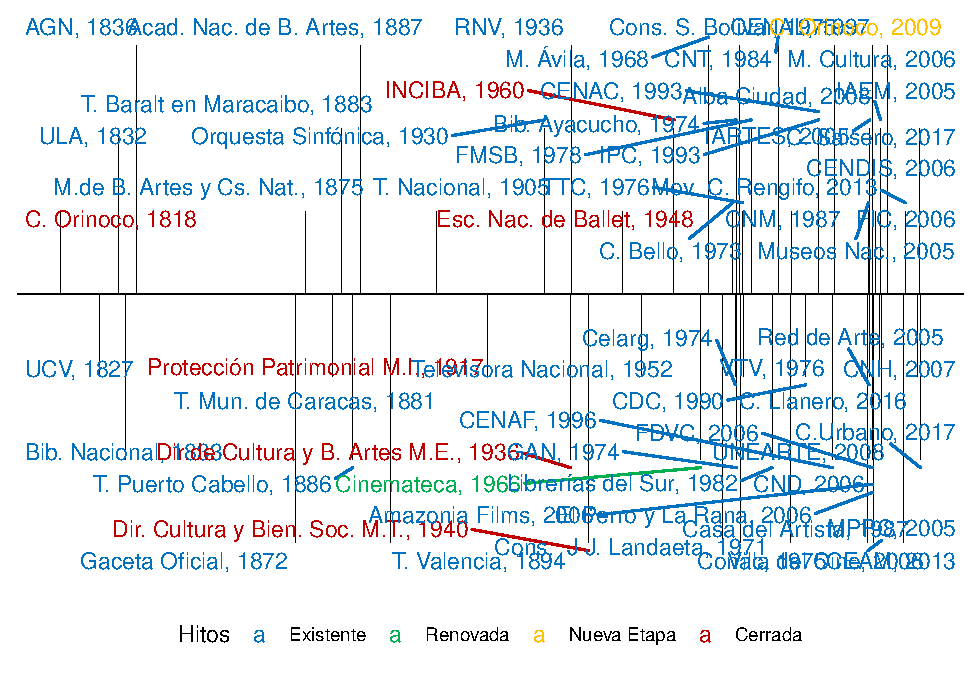
\includegraphics{LineaTiempoCultural_files/figure-latex/lineaTiempo-1.pdf}


\end{document}
